\chapter{Die Informationsrückgewinnung-Middleware-Lösung}
\label{chap:BD4B}

\section{Vorstellung}
\label{sec:VorstellungBD4B}  

In this section we describe the \ac{JBI} \ac{BC}s shipped in the ServiceMix-mt prototype this diploma thesis focuses on, and the transport protocols they support. 



ServiceMix provides \ac{HTTP} communication support in its \ac{HTTP} \ac{JBI} \ac{BC}. Its \ac{HTTP} consumer and provider endpoints are built on the \ac{HTTP} Jetty 6 server and Jakarta Commons \ac{HTTP} Client respectively, providing support for both REST and SOAP over HTTP 1.1 and 1.2 requests.

The original \ac{HTTP} \ac{BC} is extended in the ServiceMix-mt prototype to provide multi-tenant support in \cite{Muhler2012} and \cite{gomez2012}. Muhler provides an internal dynamic creation of tenant-aware endpoints in the \ac{BC}, by injecting tenant context in the \ac{JBI} endpoint's URLs \cite{Muhler2012}. Gomez provides a \ac{NMF} with tenant context information in its properties for routing in the \ac{NMR} \cite{gomez2012}. However, in this diploma thesis we must not only provide tenant isolation at the tenant level, but also isolation at the user level. We discuss this requirement in detail in Chapters \ref{chap:spec} and \ref{chap:design}.

\begin{figure}[htb]
	\centering
		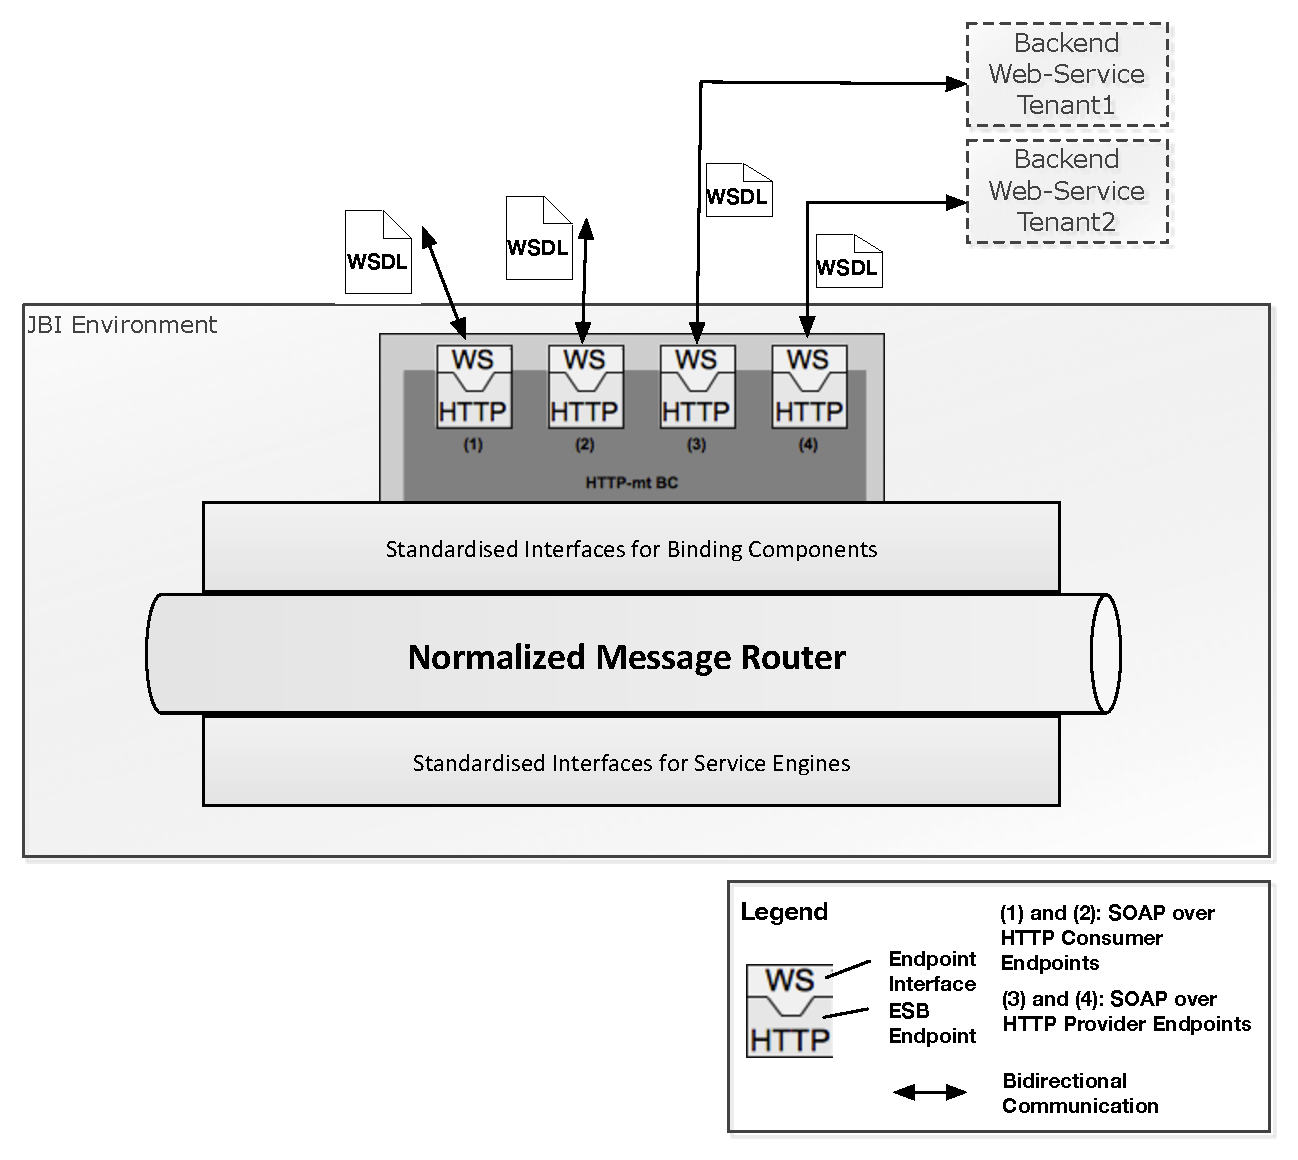
\includegraphics[clip, scale=0.3]{./gfx/httpmtbc.pdf}
	\caption[Multi-tenant HTTP Binding Component]{Multi-tenant HTTP Binding Component \cite{gomez2012}. }
	\label{fig:httpmt}
\end{figure}

As seen in Figure \ref{fig:httpmt}, the multi-tenant \ac{HTTP} \ac{BC} is mainly used in ServiceMix-mt to support the \ac{SOAP} over \ac{HTTP} communication protocol by exposing a Web service in the tenant-aware consumer endpoint and consuming an external Web service in the provider endpoint. \ac{SOAP} defines an \ac{XML} message format  which is sent over the network and a set of rules for processing the \ac{SOAP} message in the different \ac{SOAP} nodes which build the message path between two endpoints \cite{Weera2005}. A \ac{SOAP} message is a composition of three main elements: a SOAP envelope, header, and body. A SOAP envelope may contain zero or more headers and one body. The header may contain processing or authentication data for the ultimate receiver or for the intermediate nodes through the message is routed. The message payload or business data is included in the SOAP body. SOAP is used as a message framework for accessing Web services in loosely coupled infrastructures \cite{Weera2005}. The Web service consumer specifies the functionality to invoke in the SOAP body. If the Web service functionality has a request-response \ac{MEP}, a SOAP message is used to send the response data when the corresponding operation has been executed successfully or the error data in case an error occurred during execution.

Most of the Cloud storage providers provide an \ac{HTTP} interface to the tenants for data management, retrieval, and storage. In this diploma thesis we extend this \ac{JBI} \ac{BC} in order to provide the tenant a transparent access to his \ac{NoSQL} Cloud data stores.

\FloatBarrier

\section{Anforderungen}
\label{sec:AnforderungenBD4B}

The \ac{JNDI} defines a framework for deployment support in a \ac{JVM} of downloaded or extended applications known as \term{bundles}. This framework requires OSGi-friendly devices a minimum system's resources usage by providing dynamic code-loading and \term{bundle} lifecycle management. An \ac{OSGi} \term{bundle} is the packaging of a group of Java classes and required and provided capabilities' meta-data as a JAR file for providing functionality to end users. \ac{OSGi} \term{bundles} can be downloaded, extended and installed remotely or locally in the platform when needed without the need of system reboot. Installation and update of bundles during their lifecycle are also managed by the framework, which uses a service registration for selection, update notifications, or registry of new service objects offered by a deployed bundle. This feature is the main key for connecting bundles whose's services require during runtime capabilities provided by another bundles. The framework defines a bundle's requirement capability as a dependency.      

The \ac{OSGi} framework defines 5 different layers and a bundle's lifecycle \cite{OSGi2011}. An optional Security Layer provides the infrastructure for deploying and managing applications which must be controlled during runtime. The Module Layer lists the rules for package sharing between the deployed bundles. The lifecycle of a bundle can be modified during runtime through an API provided in the lifecycle layer. The main operations implemented are install, update, start, stop or uninstall. 

\subsection{Funktionelle Anforderungen}
\subsection{Nicht funktionelle Anforderungen}
\subsection{Plattformanforderungen}
\subsection{Komponentenanforderungen}
\subsection{Anforderungen an dem Ähnlichkeitsalgorithmus}
\section{High-Level Architektur}
\label{sec:HighLevelArchitektur}  

A multi-tenant management system must fulfill several requirements, such as data and performance isolation between tenants and users, authentication, specification of different user roles, resources usage monitoring, etc. In a \ac{JBI} environment, endpoint and routing configurations files are packed in \ac{SU}s, and the latter in \ac{SA}s for deployment. However, there is a lack of user-specific data during deployment. Muhler solves this problem in JBIMulti2 by injecting tenant context in the \ac{SA} packages, making them tenant-aware \cite{Muhler2012}. 

\begin{figure}[htb]
	\centering
		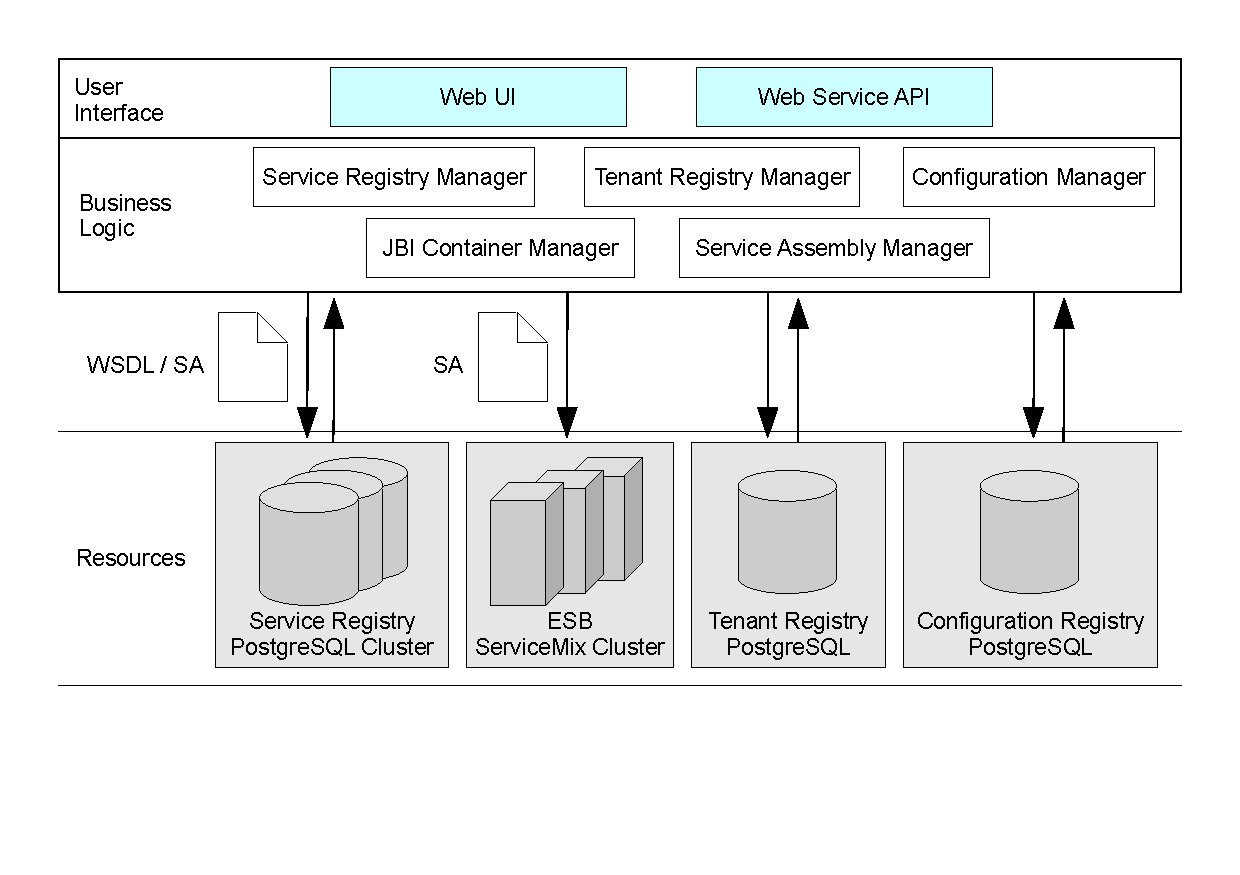
\includegraphics[clip, scale=0.5]{./gfx/systemoverview_jbimulti2.pdf}
	\caption[JBIMulti2 System Overview]{JBIMulti2 System Overview \cite{Muhler2012}} 
	\label{fig:jbimulti2}
\end{figure}

The architecture of the JBIMulti2 system is represented in Figure \ref{fig:jbimulti2}. We can distinguish two main parts in the system: business logic and resources. JBIMulti2 uses three registries for storing configuration and management data. When a tenant (or a tenant user) is registered, an unique identification number is given to them and stored in the Tenant Registry. Both Tenant Registry and Service Registry are designed for storing data of more than one deployed application. The former for storing tenant information and the latter for providing a dynamic service discovery functionality between the different applications accessed through the \ac{ESB}. The Configuration Registry is the key of the tenant isolation requirement of the system. Each of the stored tables are indexed by the tenant id  and user id value. In this thesis we need tenant information during runtime. We reuse and extend the databases schemas produced by Muhler, specifically the Service Registry.

The system provides a user interface for accessing the application's business logic. Through the business logic, the management of tenants can be done by the system administrator or the management of tenant's users can be done by the tenants. Furthermore, when deploying the different tenant's endpoint configurations packed in \ac{SA}s, the system first makes modifications in the zip file for adding tenant context information and then communicates with the Apache ServiceMix instance by using a \ac{JMS} Topic to which all the ServiceMix instances are subscribed to. The \ac{JMS} management service in ServiceMix deploys the received \ac{SA} injected in the received \ac{JMS} message using the administration functionalities provided in ServiceMix. The communication between the business layer and the ServiceMix instance is unidirectional. When successful deployment, the endpoint is reachable by the tenant. When an error occur during deployment, an unprocessed management message is posted in a dead letter queue.

JBIMulti2 requires the previous installation of components, e.g. JOnAS server, PostgreSQL, etc. The initialization of the application is described in both Chapter \ref{chap:validationevaluation} and in the JBIMulti2 setup document \cite{JBIMulti2Man}.

%\clearpage 

%In this chapter we provide a general overview on the different approaches that are taken into account in order to provide a reliable, secure, and transparent communication between on-premise application's layers and off-premise Cloud data stores. Furthermore, we discuss about the needed adaptations different authors specify that the on-premise application's layers must address when migrating their underlying layers to a Cloud infrastructure. We compare it to the ones we transparently support in our approach, and the ones the user should consider. We finally mention the improvements we need to perform to the original prototype ServiceMix-mt, and continue our discussion dividing it into the two main \ac{DBMS} available nowadays in the market: \ac{SQL} and \ac{NoSQL} databases.

%% non functional data layer patterns paper: make a big emphasis on the proxy approach. It is quite similar to our approach, because it allows horizontal scalability between different target data sources, but there is no need of abstracting the proxy from the database layer. esb's are horizontally scalable and can form a esb cluster, as described in the esb part in fundamentals. we can have in our approach a bottleneck when using one instance of the esb. furthermore, their proxy approach assumes that the database layer is in the private cloud, while in ours the database layer can reside either on or off premise.
%A migration process of the Database Layer of an application to the Cloud may pop up several incompatibilities with the new hosting environment, which need to be addressed prior to the migration decision. Strauch et al. aim to address such incompatibilities by defining a set of \term{Cloud Data Patterns}, which target finding a solution for a challenge related to the data layer of an application in the Cloud for a specific context \cite{strauchABKL2012}. Incompatibilities a user may find when migrating the application's data layer can be on the level of the schema representation, supported set of queries or query language, communication protocol, security, etc. Strauch et al. focus mainly in two non-functional aspects: enabling data store scalability and ensuring data confidentiality \cite{strauchABKL2012}. 

%The former deals with maintaining the quality of service levels when the workload increases, for both write and read operations. There are two scalability mechanisms when dealing with data: vertical and horizontal scalability. A vertical scalable system can be obtained by introducing more powerful hardware, or moving to a more powerful database system, while a horizontal scalable system deals with splitting data into groups which are stored in different partitions or different database systems, also known as \term{sharding}. Due to the absence of support for accessing a \term{sharded database} between different database systems, the concepts of a database proxy and sharding-based router are introduced. In this first approach, a proxy component is locally added below each data access layer \cite{strauchABKL2012}. A proxy below each data access layer instead of a common proxy on top of the database layer dismisses a common point of failure when accessing the data. In the second approach, a local sharding-based router is added below each of the data access layer. A sharded-based router contains the needed knowledge about the location of the \term{sharded databases}. In our approach, we don't only partially follow both of the concepts, but integrate them in a single component. We consider a sharded-based router as a proxy with routing capabilities. Therefore, as it is discussed in Chapter \ref{chap:design}, enhancing an \ac{ESB} with the required \term{sharded databases} knowledge and with standardized communication protocols, it allows us to utilize it as a sharded-based router, and as a proxy. Furthermore, the single point of failure avoidance can be ensured by increasing the number of \ac{ESB} instances and balancing the load between them. As discussed before, we do not fully comply with this approach. The development of a proxy or sharded-based router component below each data access layer forces each application to deploy at least one proxy or sharded-router instance in their system. In our approach we propose the utilization of our prototype as a shared transparent Cloud data access layer by connecting to a data access endpoint which supports a specific \ac{DBMS} multi-tenant aware communication protocol (e.g. MySQL or PostgreSQL). For this purpose, we propose the concept of a lightweight Data Layer, where the adaptations to its sublayers are minimized, e.g. modification of data access host, port, etc. The data access endpoint acts as a database protocol-aware proxy, forwarding the requests to the \ac{NMR} of the \ac{ESB}. We enhance the Myosotis Tungsten Connector and provide access control, caching functionality, and full integration in the \ac{ESB} \ac{OSGi} container, and with the \ac{NMR} \cite{tungstenwiki}.

%% Data confidentiality between the on premise app layers and the migration layers and how can we still ensure data confidentiality: mention the 5 patterns that are in steve's article. Mention that this article gives a deep focus on security patterns rather than technical information regarding the router between the data stores. we do not implement automatic data filtering for confidentiality. the user is the one who decides which data goes off premise and which data stays in premise. we provide support for off premise and on the on premise data. however, this can be reached in our esb but requires user customization, in order to be able to filter data per user and to route it to the appropriate data store.

%Ensuring data confidentiality is presented in \cite{strauch2012}. Their work deals with critical data management between on-premise and off-premise data stores, and categorizes data into different confidentiality levels to prevent data disclosures. The former is achieved by aggregating information which categorizes data into different categories and confidentiality levels. The latter deals with keeping confidential data on-premise. With data filtering, pseudonymization, and anonymization, data is either prevented from being externally routed, or secured when routed to a public Cloud \cite{strauch2012}. The pseudonymization technique provides to the exterior a masked version of the data while maintaining its relation with the original data, and the anonymization provides to the exterior a reduced version of the data. In this diploma thesis' approach, we assume that the application's owner has decided on which data should be and cannot be migrated, and that the business layer is hosted on-premise. Therefore, there is no data processing in a public Cloud environment. Our final prototype provides confidentiality between different tenants of the system by injecting tenant information  in our messages and providing tenant-aware routing, and different multi-tenant aware endpoints. We do not need to provide support for pseudonymization or anonymization techniques, in contrast to \cite{strauch2012}.

%% table of what do i have to do when migrating app or app components to the cloud. this is from the book chapter of vasilios and steve. comment here what ive written in the comments
%Replacement of components which build an application with Cloud offerings leads the developers to face an application's adaptation process. For example, migrating a local database to a private Cloud or to a public Cloud, or sharding a database between on-premise and off-premise data stores forming a single data store system, can not be accessible without adapting the non-migrated application's layers to the new storage system. Andrikopoulos et al. identify the needed adaptations actions when migrating a data layer to the Cloud \cite{andrikopoulos2013}: address reconfiguration, patterns realization, incompatibilities resolution, query transformation, and interaction with data store allowance. Our main goal in our final prototype is to minimize the number of adaptations the user must perform when migrating application's data to a Cloud data store. The adaptations of the \ac{ESB} must encompass the described adaptations in a transparent way to the user, in order to internally support in our prototype compatibility between the application and the different data stores, and lower the adaptation operations number at the application's side, e.g. only address reconfiguration. 

%% speak a little bit about federated databases
%% have taken notes in the paper. the main thing to say here is the main difference between a federated database system and our approach. Our approach works more or less than a federated database system, but more like a federated server, where transparent access to backend datasources is provided. joins are out of the scope of the thesis. indicate that one main component in a federated dbs is the transformer, in our case between sql databases, and between nosql databases, but this is out of scope of this thesis. 
%% mediator in page 37 of the book principles of distributed database systems
%Federated Database Systems are a type of \ac{MDBS} that allow accessing and storing data which is stored in different and noncontiguous databases through a single interface. Sheth and Larson define them as a collection of cooperating but autonomous component database systems, which can be integrated to various degrees, and can be accessed by a software which controls and coordinates the manipulation of the database systems which conforming the federated database system. This distributed database model allows users to access and store data among different database systems, which can be located in different continents, without dealing with multiple connections to the different database systems, query and data transformation, address adaptation, etc. \ac{MDBS} are accessed through a single endpoint which provides a single logical view of the \ac{MDBS}, and users can access the different \ac{DBMS} which form the \ac{MDBS} (see Figure \ref{fig:multidatabasesystem}). 

%\begin{figure}[htb]
%	\centering
%		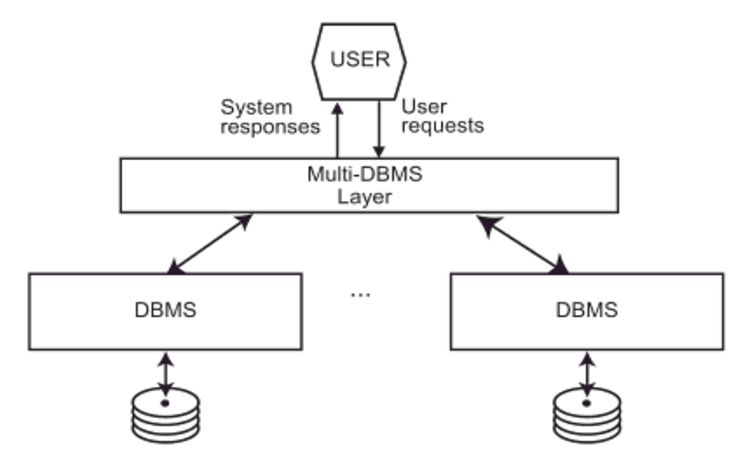
\includegraphics[clip, scale=0.6]{./gfx/multidatabasesystem.pdf}
%	\caption[Multidatabase System Components]{Components in a multidatabase %system \cite{ddbsozsu}}
%	\label{fig:multidatabasesystem}
%\end{figure}

%A popular implementation architecture for a \ac{MDBS} is the mediator/wrapper approach \cite{ddbsozsu}. Mediators exploits knowledge to create information for upper layers, while wrappers provide mapping between different views, e.g. relational vs. object-oriented views. We can consider our approach as a \ac{MDBS} with some modifications and less functionalities. In the first place, using the \ac{ESB} as a single entrance point to the data system while managing different backend autonomous Cloud or traditional data stores comply with the main concept of a \ac{MDBS}. Furthermore, Cloud data store providers may implement the same distributed database model, whereby we could find two logical levels for accessing the physical data. However, we do not accurately follow the mediator/wrapper approach. In our approach we exploit data provided by the tenant during the migration decision and process, by providing an interface to register the backend data store/s information in our system, for future routing purposes. Furthermore, compatibility information is registered in order to apply the needed query or data transformation between data stores. However, the transformation is out of the scope of this diploma thesis, and the support of table joins between databases located in different Cloud data stores are out of scope as well.
%%tenant isolation approach in muhler versus tenant and user isolation approach in this work. explain the granularity of tenant and users, one tenant may want to migrate his database to a data store, but in this case one database can have one or more users. it is not like in muhlers approach where tenants are considered applications accessing the esb. 

%As described in the previous chapter, multi-tenancy is one of the main requirements in a Cloud environment. Muhler, Essl, and Gomez provide an extended version of ServiceMix 4.3, which supports multi-tenancy at two different levels: communication, and administration and management \cite{Muhler2012}, \cite{Essl2011}, \cite{gomez2012}. However, their prototype supports tenant isolation at the level of tenants. A \ac{DBMS}, e.g. MySQL, by default provides access to one default user and supports multiple users creation \cite{mysqlmanual}. Therefore, in our approach we must not only consider isolation at the tenant level, but also at the user level. We assume that the tenant is the default user which migrates his data store to a Cloud environment, but the migrated data store may contain one or more users. In our prototype we ensure tenant and user isolation at both communication, and administration and management levels.

%% caching mechanism used in our approach, explaining the two levels of caching that we use. compare it to the actual mysql proxy and to the databases architectures in the cloudcomputingdatabaseapps paper, say that caching is not discussed in their approach. caching applies for both mysql and nosql. drivers provided by the different vendors do not provide caching functionality. caching functionality must be trated in the application or in the server. caching is good not only for performance, but also to give the possibility to reduce costs in the tenants data stores in the cloud. most of the providers dont only charge per storage size, but also per calls to their api
%%mention the paper
%% put examples on amazon pricing : Micro DB Instance	$0.025 Small DB Instance	$0.090 Medium DB Instance	$0.180 Large DB Instance	$0.365 Extra Large DB Instance	$0.730 this are prices of usage per hour
%% amazon dynamo db: Write Throughput: $0.01 per hour for every 10 units of Write Capacity - Read Throughput: $0.01 per hour for every 50 units of Read Capacity
%% google cloud storage: (per 1,000 requests/month) PUT, POST, GET bucket**, GET service** Requests $0.01 - GET, HEAD Requests (per 10,000 requests/month) $0.01 - DELETE Requests free
%Over the past decades, caching has become the key technology in bridging the performance gap across memory hierarchies via temporal or spatial localities; in particular, the effect is prominent in disk storage systems \cite{cashing2012}. Han et al. investigate how cost efficiency in a Cloud environment can be achieved, specially in applications which require a high I/O activities number, and present a CaaS (cache-as-a-service) model. Cloud providers offering data storage solutions present pricing models based on the storage size, usage per time, or number of requests. Amazon RDS costs \$0.025 per hour for a Micro DB Instance usage  \cite{amazonrds}, while Amazon DynamoDB \$0.01 per hour for every 50 units of read capacity \cite{amazondynamodb}, and Google Cloud Storage \$0.01 per 1000 PUT, POST, GET requests per month \cite{googlecloudstorage}. An I/O-intensive application whose database is hosted in the Cloud may produce a significant economic cost. The cost of continuously retrieving data from the Cloud data store, when existing temporal proximity between the data accessed, can be considered unnecessary, and reducible. Furthermore, the application's overall performance can be reduced due to the network latency and, in the scope of this work, the use of an \ac{ESB} to access the Cloud data store. In this diploma thesis we do not provide cashing as a service, but include cashing support to the sharded-based router pattern described in \cite{strauchABKL2012}. Uralov enhaces ServiceMix-mt with cashing support for dynamic discovery and selection of Cloud data hosting solutions \cite{Uralov2012}. However, we must adapt and extend it due to the lack of support of functionalities we require and the lack of full \ac{OSGi} compliance. 

 